\documentclass{beamer}

\usepackage[italian]{babel}
\usepackage[utf8]{inputenc}
\usepackage{graphicx}
\usepackage{subfig}
\usepackage{hyperref}

\title{Introduzione a \texttt{git}}
\author{Luca Tagliavini, Stefano Volpe}
\institute{Università di Bologna, corso di Laurea in Informatica}
\date{8 novembre 2022}
\logo{
\includegraphics[width=0.05\textwidth]{assets/by-nc-sa-4-0.png}}

\AtBeginSection[]{
  \begin{frame}
    \frametitle{In questa sezione}
    \setcounter{tocdepth}{2}
    \tableofcontents[currentsection]
  \end{frame}
}

\begin{document}

\begin{frame} 
  \titlepage
\end{frame}

\section{Controllo di versione}

\subsection{Problemi e rimedi}
\begin{frame}{Problemi}
  Quando lavoriamo con molti \emph{file} (redigiamo documenti, creiamo arte
  digitale, scriviamo codice...), ricorrono alcuni \textbf{problemi}:\pause
  \begin{itemize}
    \item<1-> mantenere una \textbf{cronologia} delle modifiche;\pause
    \item<2-> \textbf{ripristinare} subito un qualsiasi stato precedente;\pause
    \item<3-> collaborare a \textbf{copie diverse} dello stesso progetto.\pause
  \end{itemize}
  Copie di cartelle e blocchi note condivisi in rete non bastano più!
\end{frame}

\begin{frame}{Rimedi}
  \begin{block}{Definizione}
    Un \textbf{sistema per il controllo di versione} (o VCS, \emph{version control
    system}) è un applicativo che gestisce modifiche a grandi insiemi di
    informazioni.
  \end{block}\pause
  \begin{figure}
    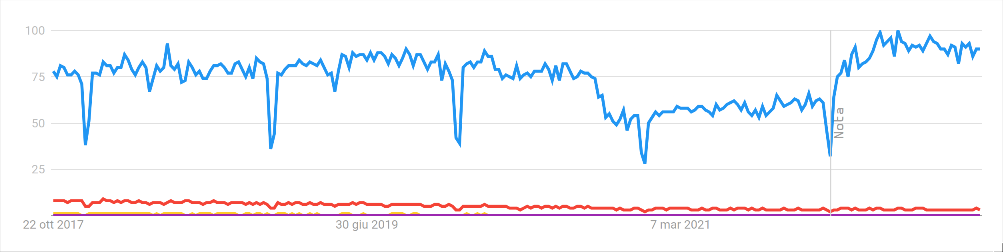
\includegraphics[width=\textwidth]{assets/vcs-popularity.png}
    \caption{popolarità su Google dei cinque principali VCS
    (\textcolor{cyan}{\texttt{git}}, \textcolor{red}{SVN},
    \textcolor{orange}{Mercurial}, \textcolor{green}{Perforce},
    \textcolor{violet}{CVS}) negli ultimi cinque anni. In ordinata, 100 indica il
    massimo storico del più popolare di questi in tale lasso di tempo.}
  \end{figure}
\end{frame}

\subsection{Ambiente di lavoro}
\begin{frame}{Ambiente di lavoro | Scopo}
  Nei prossimi lucidi, collegandoci alle macchine di laboratorio con i nostri
  utenti, useremo \texttt{git} da linea di comando.\pause
  \begin{block}{Consiglio}
    Tenete aperta questa presentazione anche sulla vostra macchina durante il
    laboratorio: potete trovarla su
    \href{https://csunibo.github.io/lab}{\beamergotobutton{csunibo.github.io/lab}}.
  \end{block}
\end{frame}

\begin{frame}{Ambiente di lavoro | Materiali}
  Materiali:
  \begin{enumerate}
    \item<1->un utente nella rete dipartimentale (es. \texttt{stefano.volpe2});
      \begin{alertblock}{Se siete senza utente...}
        ... (e non avete \texttt{git} neanche sulla vostra macchina), seguite con
        chi siede al vostro fianco.
      \end{alertblock}\pause
    \item<2->un client \texttt{ssh}. Su Linux e macOS è già installato; su
      Windows, se vi manca, c'è
      \href{https://www.chiark.greenend.org.uk/~sgtatham/putty/latest.html}{\beamergotobutton{PuTTY}};
    \item<3->un utente su una piattaforma di \emph{hosting} per progetti
      \texttt{git}.
  \end{enumerate}
\end{frame}

\begin{frame}{Ambiente di lavoro | Preparazione}
  Preparazione:
  \begin{enumerate}
    \item<1->scegliere una delle \href{https://disi.unibo.it/it/dipartimento/servizi-tecnici-e-amministrativi/servizi-informatici/accesso-remoto}{\beamergotobutton{macchine
      di laboratorio}} (es. \texttt{XXX.cs.unibo.it}, dove \texttt{XXX} è il
      nome della macchina scelta)
    \item<2-> collegarsi:
      \begin{semiverbatim}
        \$ ssh stefano.volpe2@XXX.cs.unibo.it
      \end{semiverbatim}
  \end{enumerate}
\end{frame}

\begin{frame}{Ambiente di lavoro | Preparazione (2)}
  \begin{semiverbatim}
  \lbrack ...\rbrack \newline
  Are you sure you want to continue connecting \newline (yes/no/\lbrack
  fingerprint\rbrack)? yes \newline
  \lbrack ...\rbrack \newline
  stefano.volpe2@XXX.cs.unibo.it's password:
  \end{semiverbatim}
\end{frame}

\begin{frame}{Ambiente di lavoro | Preparazione (3)}
  \begin{enumerate}
    \setcounter{enumi}{2}
    \item configurare \texttt{git} con i vostri dati:
    \begin{semiverbatim}
    \$ git config --global user.name "Stefano Volpe"
    \end{semiverbatim}
    \begin{semiverbatim}
    \$ git config --global user.email \\
    \end{semiverbatim}
    \begin{semiverbatim}
        \qquad"stefano.volpe2@studio.unibo.it"
    \end{semiverbatim}
  \item generare una chiave ssh:
    \begin{semiverbatim}
    \$ ssh-keygen -t ed25519 -C \\
    \end{semiverbatim}
    \begin{semiverbatim}
        \qquad"stefano.volpe2@studio.unibo.it"
    \end{semiverbatim}
  \end{enumerate}
\end{frame}

\section{Basi di \texttt{git}}

\subsection{\texttt{git init, status}}
\begin{frame}{\texttt{git init}}
  \begin{block}{Definizione}
    Una \emph{repository} è un progetto manutenuto con \texttt{git}.
  \end{block}\pause

  Per inizializzare una \emph{repository} Git vuota in una nuova cartella
  \texttt{<directory>}:
  \begin{semiverbatim}
  \$ git init [<directory>]
  \end{semiverbatim}
  \begin{block}{Nota}
    I file interni di \texttt{git} sono nella sottocartella
    \texttt{<directory>/.git/}
  \end{block}
  \begin{block}{Nota 2}
    Se \texttt{<directory>} non è specificata, viene
    usata la cartella corrente.
  \end{block}
\end{frame}

\begin{frame}{Stati dei \emph{file}}
  I \emph{file} di una \emph{repository} sono sempre in esattamente uno dei
  seguenti quattro stati:
  \begin{enumerate}
    \item<1->\emph{untracked} (non tracciato da \texttt{git});
    \item<2->\emph{unmodified} (non modificato rispetto all'ultima
      "istantanea" di \texttt{git});
    \item<3->\emph{modified} (modificato rispetto all'ultima
      "istantanea" di \texttt{git});
    \item<4->\emph{staged} (modificato rispetto all'ultima "istantanea" di
      \texttt{git} e pronto a essere registrato).
  \end{enumerate}
\end{frame}

\begin{frame}{\texttt{git status}}
  \begin{figure}
    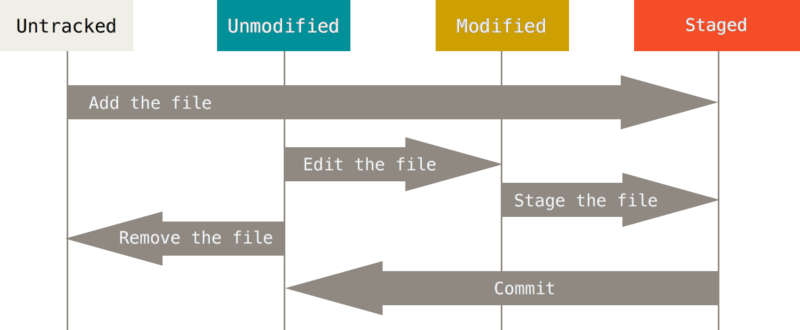
\includegraphics[width=0.75\textwidth]{assets/lifecycle.png}
    \caption{Gli stati fra cui i \emph{file} di una \emph{repository} si
    muovono. \href{https://git-scm.com/book/en/v2/Git-Basics-Recording-Changes-to-the-Repository}{\emph{Pro Git},
    figura 8} di Scott Chacon e Ben Straub, rilasciata sotto licenza
    \href{https://creativecommons.org/licenses/by-nc-sa/3.0/}{CC
    BY\_NC\_SA 3.0}.}
  \end{figure}\pause
  Con \texttt{git status}, mostriamo lo stato attuale del nostro "albero di
  lavoro".
\end{frame}

\begin{frame}{\texttt{.gitignore}}
  Si possono ignorare file che non si desiera vengano aggiunti alla
  \emph{repository}, come binari compilati e file di caching, elencandoli in un
  file denominato \texttt{.gitignore} situato nella radice dell'albero di
  lavoro. \\
  La sintassi \`e dettata dalle seguenti regole:
  \begin{enumerate}
    \item una riga contiene il percorso ad un file da ignorare;
    \item si possono usare raggruppamenti \emph{glob} per selezionare pi\`u file
      in modo conciso;
    \item iniziando la linea con un \texttt{!} il file viene \textbf{incluso}
      anche se ignorato.
  \end{enumerate}
\end{frame}

\subsection{\texttt{git add, commit}}
\begin{frame}{\texttt{git add}}
  \begin{figure}
    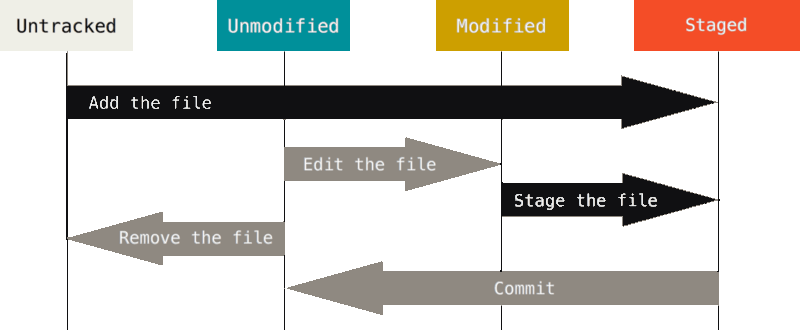
\includegraphics[width=0.75\textwidth]{assets/lifecycle-add.png}
    \caption{Gli stati fra cui i \emph{file} di una \emph{repository} si
    muovono. \href{https://git-scm.com/book/en/v2/Git-Basics-Recording-Changes-to-the-Repository}{\emph{Pro Git},
    figura 8} di Scott Chacon e Ben Straub, rilasciata sotto licenza
    \href{https://creativecommons.org/licenses/by-nc-sa/3.0/}{CC
    BY\_NC\_SA 3.0} / Parz. ricolorata.}
  \end{figure}
  Aggiunge \texttt{<pathspec>} (non tracciato o modificato) agli
  \emph{staged files}:
  \begin{semiverbatim}
    \$ git add [<pathspec>...]
  \end{semiverbatim}
\end{frame}

\begin{frame}{\texttt{git commit}}
  \begin{figure}
    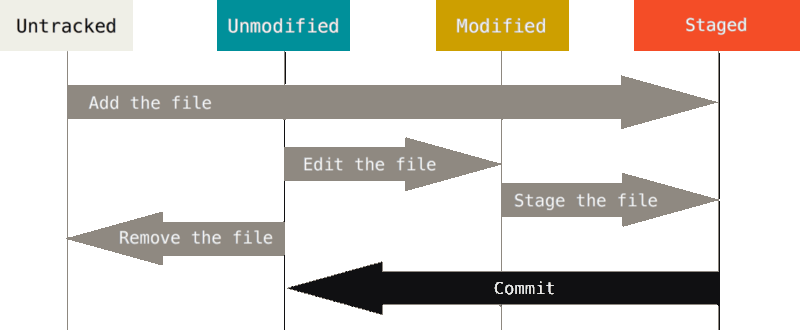
\includegraphics[width=0.75\textwidth]{assets/lifecycle-commit.png}
    \caption{Gli stati fra cui i \emph{file} di una \emph{repository} si
    muovono. \href{https://git-scm.com/book/en/v2/Git-Basics-Recording-Changes-to-the-Repository}{\emph{Pro Git},
    figura 8} di Scott Chacon e Ben Straub, rilasciata sotto licenza
    \href{https://creativecommons.org/licenses/by-nc-sa/3.0/}{CC
    BY\_NC\_SA 3.0} / Parz. ricolorata.}
  \end{figure}
  Registra le modifiche agli \emph{staged files} commentadole con \texttt{msg}:
  \emph{staged files}:
  \begin{semiverbatim}
    \$ git commit [--amend] [-m <msg>]
  \end{semiverbatim}
\end{frame}

\begin{frame}{\texttt{git commit}}
  \begin{block}{Nota}
    Se non uso \texttt{-m}, viene aperto un \emph{buffer} di testo in cui posso
    specificare il messaggio.
  \end{block}
  \begin{block}{Nota 2}
    Con \texttt{--amend}, correggo nome e/o contenuti del \emph{commit}
    precedente.
  \end{block}
\end{frame}
\subsection{\texttt{git log, show}}
\begin{frame}{\texttt{git log}}
  Mostriamo il registro dei \emph{commit}:
  \begin{semiverbatim}
    \$ git log [--graph]
  \end{semiverbatim}
  Se aggiungiamo \texttt{--graph}, il registro è rappresentato come grafo.
\end{frame}

\begin{frame}{\texttt{git show}}
  Possiamo mostrare dettagli su uno o più \emph{commit} a scelta:
  \begin{semiverbatim}
    \$ git show [<object> ...]
  \end{semiverbatim}
  Un modo di riferirsi a un \texttt{<object>} è un prefisso univoco del codice
  \texttt{sha1} del \emph{commit}. \pause Se non si specifica nulla, viene usato
  \texttt{HEAD}, il \emph{commit} corrente.
\end{frame}

\subsection{\texttt{git branch, checkout}}
\begin{frame}{\texttt{git branch, checkout }}
  Per evitare confusione, vogliamo mantenere più versioni dello stesso progetto:
  \begin{itemize}
    \item quella "buona";
    \item quella su cui stiamo sviluppando una funzione ancora sperimentale;
    \item quella su cui stiamo correggendo un problema...
  \end{itemize}\pause
  In \texttt{git}, ogni versione (\emph{branch}, ramificazione) si alterna
  nella stessa cartella.
  \begin{semiverbatim}
    \$ git branch \# elenca le branch
  \end{semiverbatim}
\end{frame}

\begin{frame}{\texttt{git branch, checkout}}
  \begin{semiverbatim}
    \$ git checkout -b <branch> \# crea <branch> e vi si sposta
  \end{semiverbatim}
\end{frame}

\begin{frame}{\texttt{git branch, checkout}}
  \begin{figure}
    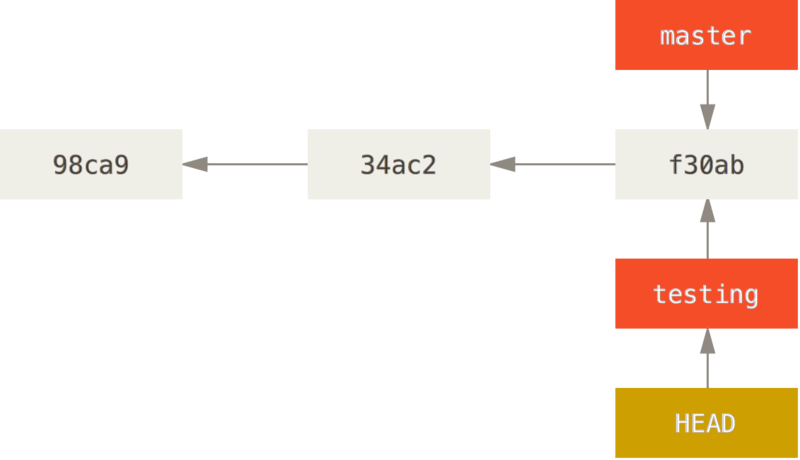
\includegraphics[width=\textwidth]{assets/head-to-testing.png}
    \caption{
      \href{https://git-scm.com/book/en/v2/Git-Branching-Branches-in-a-Nutshell}{\emph{Pro Git},
      figura 14} di Scott Chacon e Ben Straub, rilasciata sotto licenza
      \href{https://creativecommons.org/licenses/by-nc-sa/3.0/}{CC
      BY\_NC\_SA 3.0} / Testo modificato.
    }
  \end{figure}
\end{frame}

\begin{frame}{\texttt{git branch, checkout}}
  \begin{figure}
    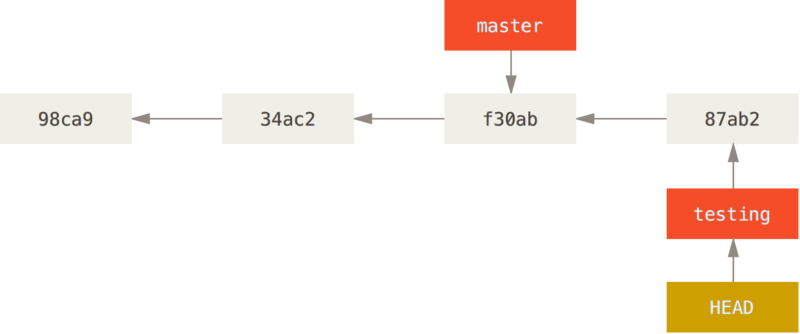
\includegraphics[width=\textwidth]{assets/advance-testing.png}
    \caption{
      \href{https://git-scm.com/book/en/v2/Git-Branching-Branches-in-a-Nutshell}{\emph{Pro Git},
      figura 15} di Scott Chacon e Ben Straub, rilasciata sotto licenza
      \href{https://creativecommons.org/licenses/by-nc-sa/3.0/}{CC
      BY\_NC\_SA 3.0} / Testo modificato.
    }
  \end{figure}
\end{frame}

\begin{frame}{\texttt{git branch, checkout}}
  \begin{semiverbatim}
    \$ git checkout <branch> \# si sposta su branch
  \end{semiverbatim}
\end{frame}

\begin{frame}{\texttt{git branch, checkout}}
  \begin{semiverbatim}
  \begin{figure}
    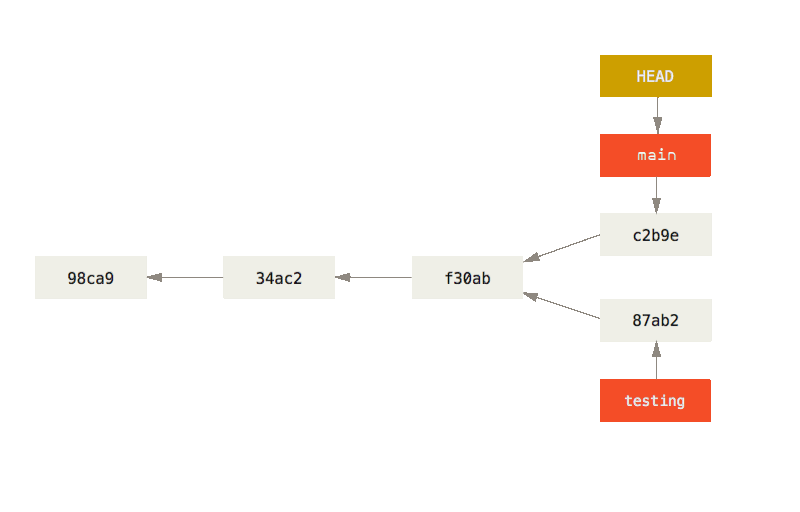
\includegraphics[width=\textwidth]{assets/advance-main.png}
    \caption{
      \href{https://git-scm.com/book/en/v2/Git-Branching-Branches-in-a-Nutshell}{\emph{Pro Git},
      figura 17} di Scott Chacon e Ben Straub, rilasciata sotto licenza
      \href{https://creativecommons.org/licenses/by-nc-sa/3.0/}{CC
      BY\_NC\_SA 3.0} / Testo modificato.
    }
  \end{figure}
  \end{semiverbatim}
\end{frame}

\begin{frame}{\texttt{git branch, checkout}}
  \begin{semiverbatim}
    \$ git branch -d <branch> \# rimuove <branch>
  \end{semiverbatim}
\end{frame}

\begin{frame}[c]
  \centering
  Pausa
\end{frame}

\subsection{\texttt{git merge, rebase}}
\begin{frame}
  \frametitle{\texttt{git merge, rebase}}
  Per unire il lavoro svolto su branch separate si hanno due opzioni che operano
  in modo diverso ed hanno casi d'uso separati:
  \begin{enumerate}
    \item<1-> \texttt{git merge <name>}: applica tutti i \emph{nuovi commit}\footnotemark{}
      presenti sulla branch \texttt{<name>} nella branch in cui ci troviamo;
    \item<2-> \texttt{git rebase <name>}: mette da parte i
      \emph{nuovi commit}\footnotemark[\value{footnote}], avanza la branch
      all'ultimo commit su \texttt{<name>} e riapplica i commit "messi da parte".
  \end{enumerate}
      \footnotetext{Tutti quelli a partire dal \emph{fork-point}}
\end{frame}

\begin{frame}
  \frametitle{\texttt{git merge} | Pregi e difetti}
  \begin{itemize}
    \item pregi: \begin{itemize}
      \item preserva \emph{chiaramente} la storia dei commit;
      \item pu\`o essere usato su branch pubbliche.
    \end{itemize}
    \item difetti: \begin{itemize}
      \item aggiunge un nuovo commit alla storia;
      \item tutti i commit della branch vengono condensati in uno\footnote{
          Sar\`a comunque possibile visionare tutti i commit della branch unita,
          anche dopo la sua rimozione.
        }.
    \end{itemize}
  \end{itemize}

  Da usare quando si collabora con altre persone e si vuole rendere la storia
  dei cambiamenti facilmente comprensibile.
\end{frame}

\begin{frame}
  \frametitle{\texttt{git rebase} | Pregi e difetti}
  \begin{itemize}
    \item pregi: \begin{itemize}
      \item non crea commit aggiuntivi, rende la storia lineare;
      \item si possono compiere modifiche ai commit precedenti durante l'unione
        delle due branch.
    \end{itemize}
    \item difetti: \begin{itemize}
      \item non \`e possibile collegare i commit riapplicati a quelli originali;
      \item \textbf{non} pu\`o essere usato su branch pubbliche;
      \item pu\`o sovrascrivere la storia e di conseguenza potrebbe
        richiedere un \texttt{push} forzato.
    \end{itemize}
  \end{itemize}

  Torna utile quando si lavora in locale o su branch private, per coprire i
  propri sbagli o ripulire una storia dei commit poco ordinata.
\end{frame}

\begin{frame}
  \frametitle{\texttt{git merge}}
  Il caso d'uso tipico per il comando \texttt{merge} \`e l'unione di una branch
  secondaria con quella principale. Il comando ha la seguente sintassi:
  \begin{semiverbatim}
  \$ git merge <branch>
  \end{semiverbatim}

  \begin{figure}
  \only<1>{
    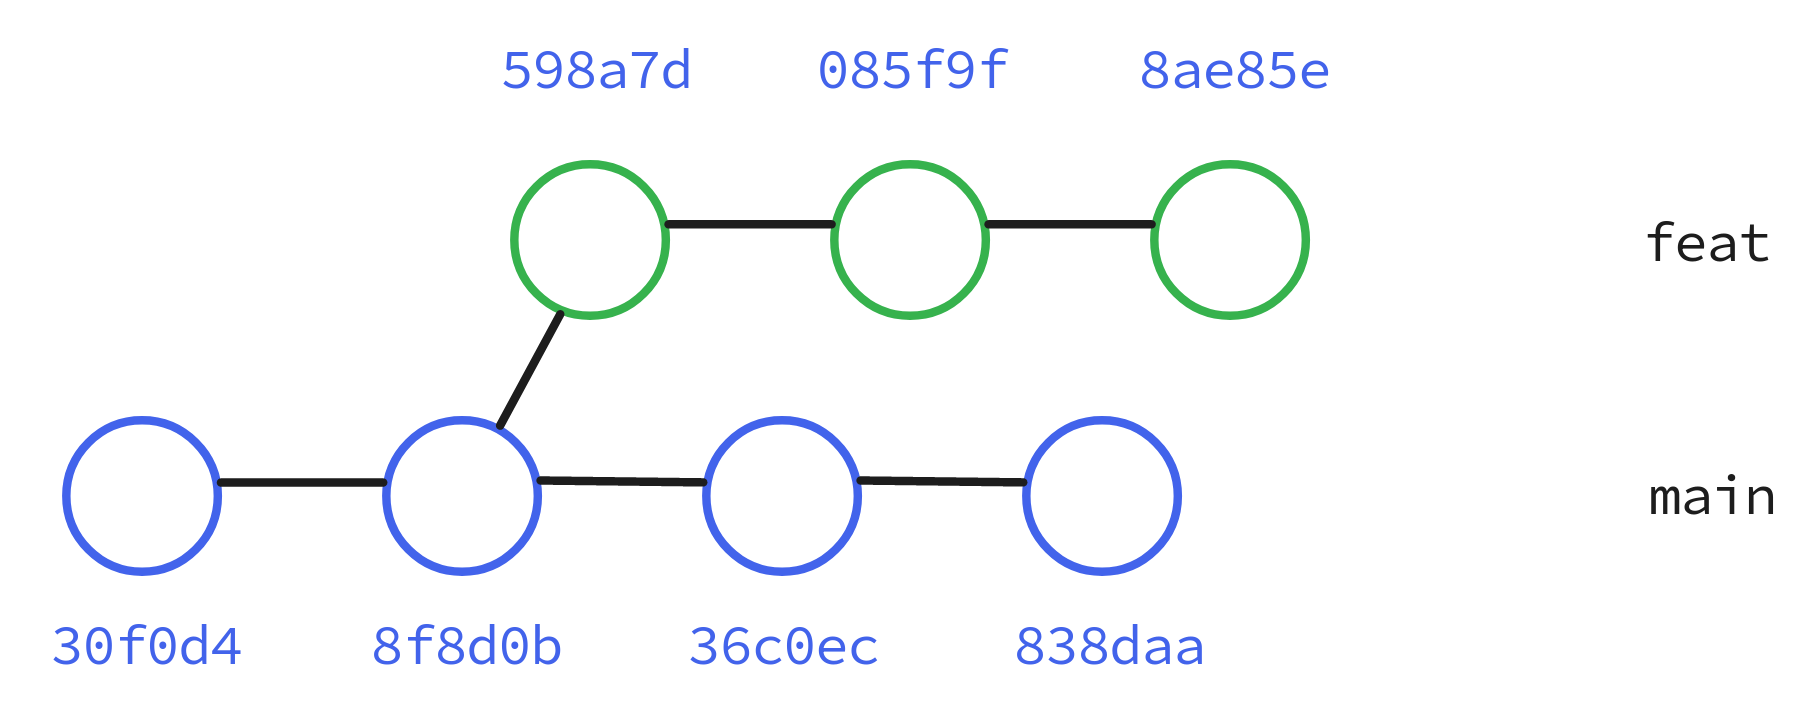
\includegraphics[width=5cm]{assets/pre-merge.png}
    \caption{Log dei commit prima di un merge}
  }
  \only<2>{
    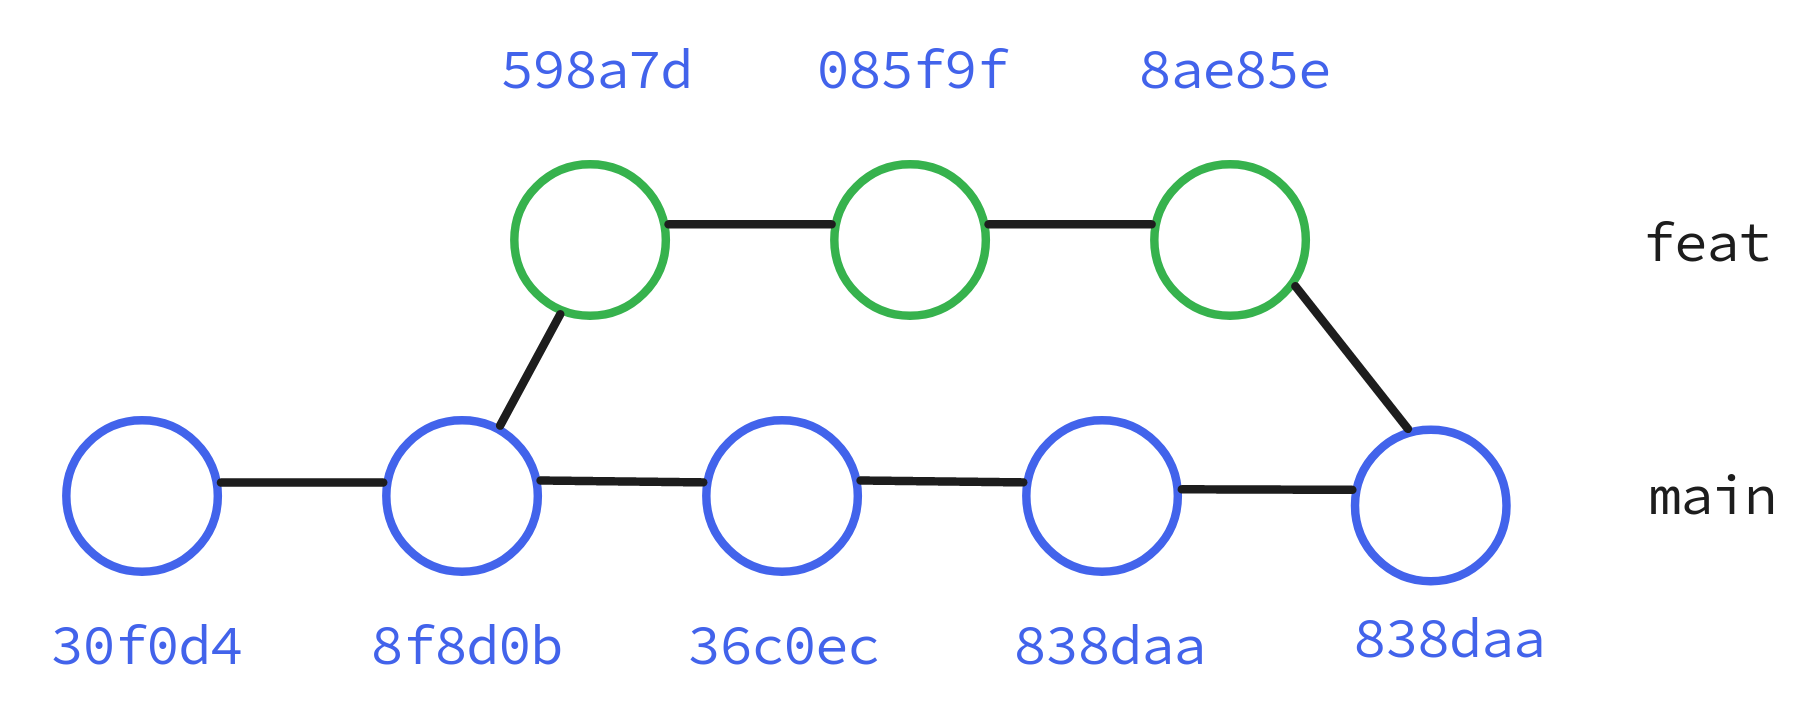
\includegraphics[width=5cm]{assets/post-merge.png}
    \caption{Log dei commit dopo $git merge feat$}
  }
  \end{figure}

  \pause
  \begin{block}{Nota}
    \`E sconsigliato usare \texttt{merge} con un spazio di lavoro sporco
  \end{block}
\end{frame}

\begin{frame}
  \frametitle{\texttt{git rebase}}
  Il comando \texttt{rebase} si usa quando si vuole cambiare il ramo su cui si
  basa la branch attuale. Tipicamente questo si rende necessario perch\`e il
  ramo su cui ci si basa \`e stato unito con la branch di sviluppo principale.
  La sintassi \`e la seguente:
  \begin{semiverbatim}
  \$ git rebase <branch>
  \end{semiverbatim}
  Di seguito \`e raffigurata una casistica d'esempio.

  \begin{figure}
  \only<1>{
    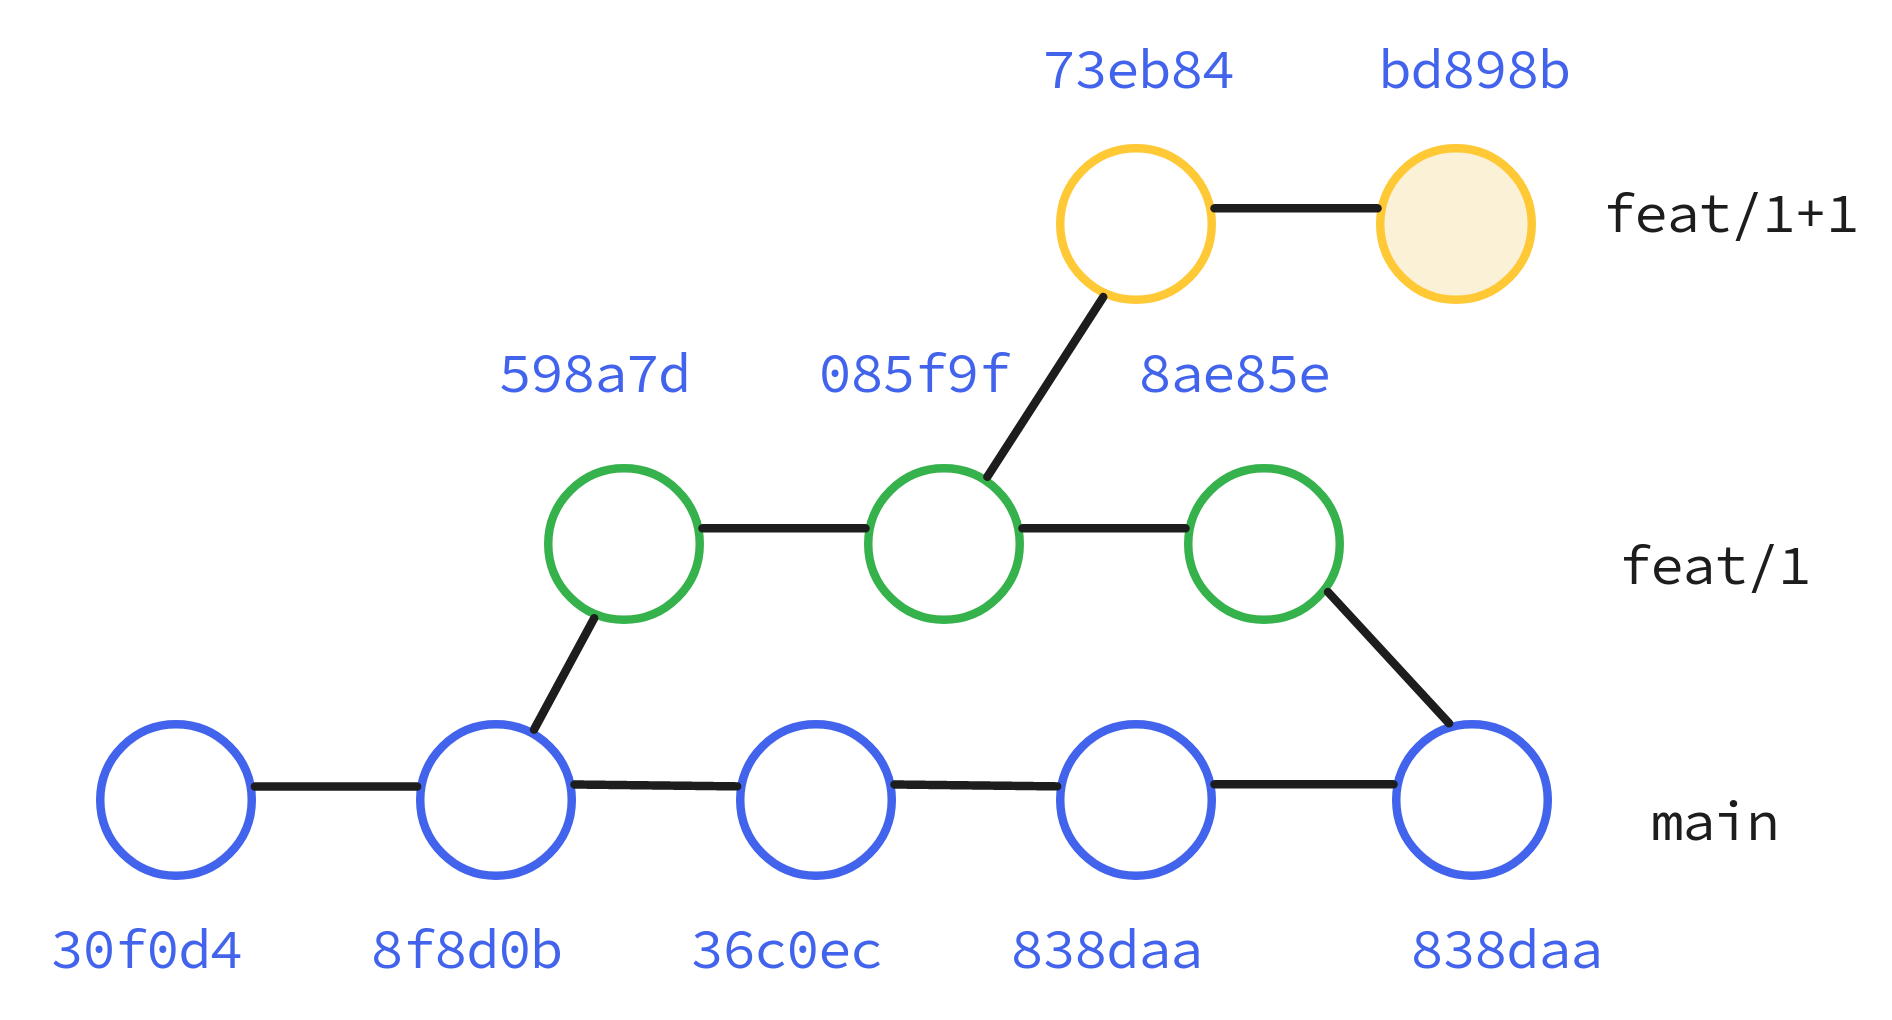
\includegraphics[width=5cm]{assets/pre-rebase.png}
    \caption{Log dei commit prima di un rebase}
  }
  \only<2>{
    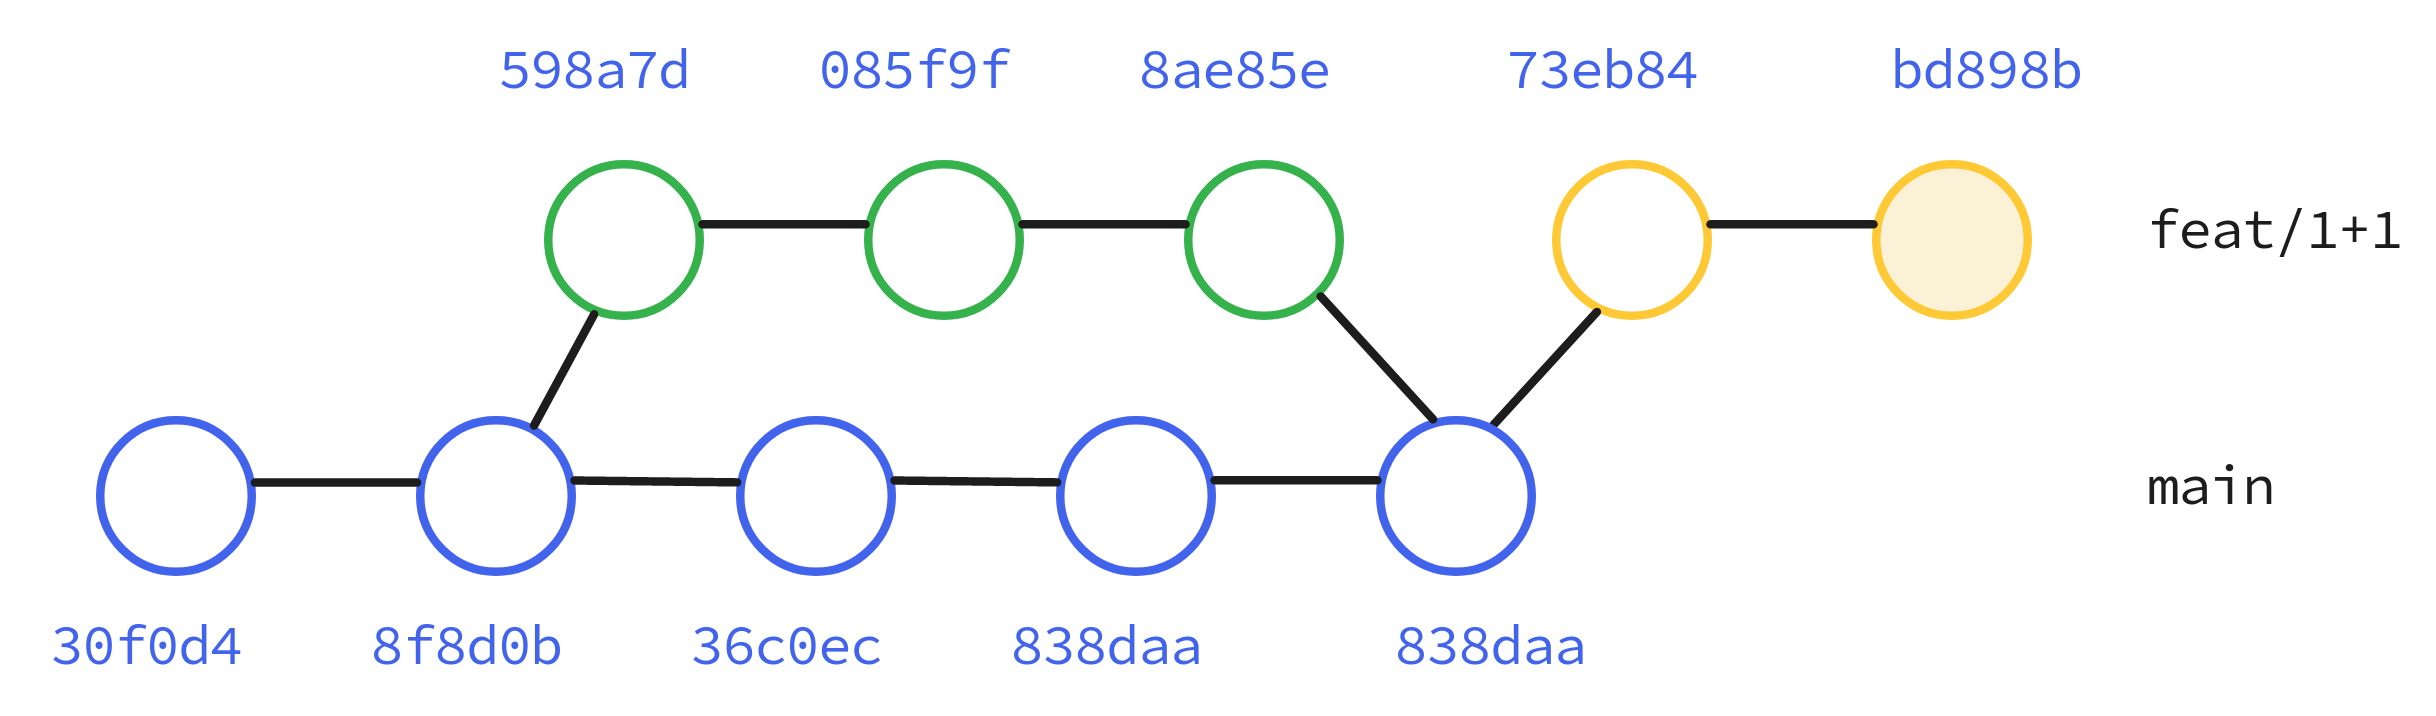
\includegraphics[width=7cm]{assets/post-rebase.png}
    \caption{Log dei commit dopo \texttt{git rebase main}}
  }
  \end{figure}
\end{frame}

\begin{frame}
  \label{trivial}
  \frametitle{\texttt{git merge, rebase} | Caso triviale}
  In un caso triviale, ovvero quando tra le branch da unificare solo una contiene
  cambiamenti dopo il \emph{fork-point}, i comandi \texttt{merge} e \texttt{rebase}
  hanno lo stesso effetto\footnote{Nel caso del \texttt{merge} non viene
  aggiunto nessun commit, si dice che viene fatto un \emph{fast forward}}:
  \begin{figure}
    \centering
    \subfloat{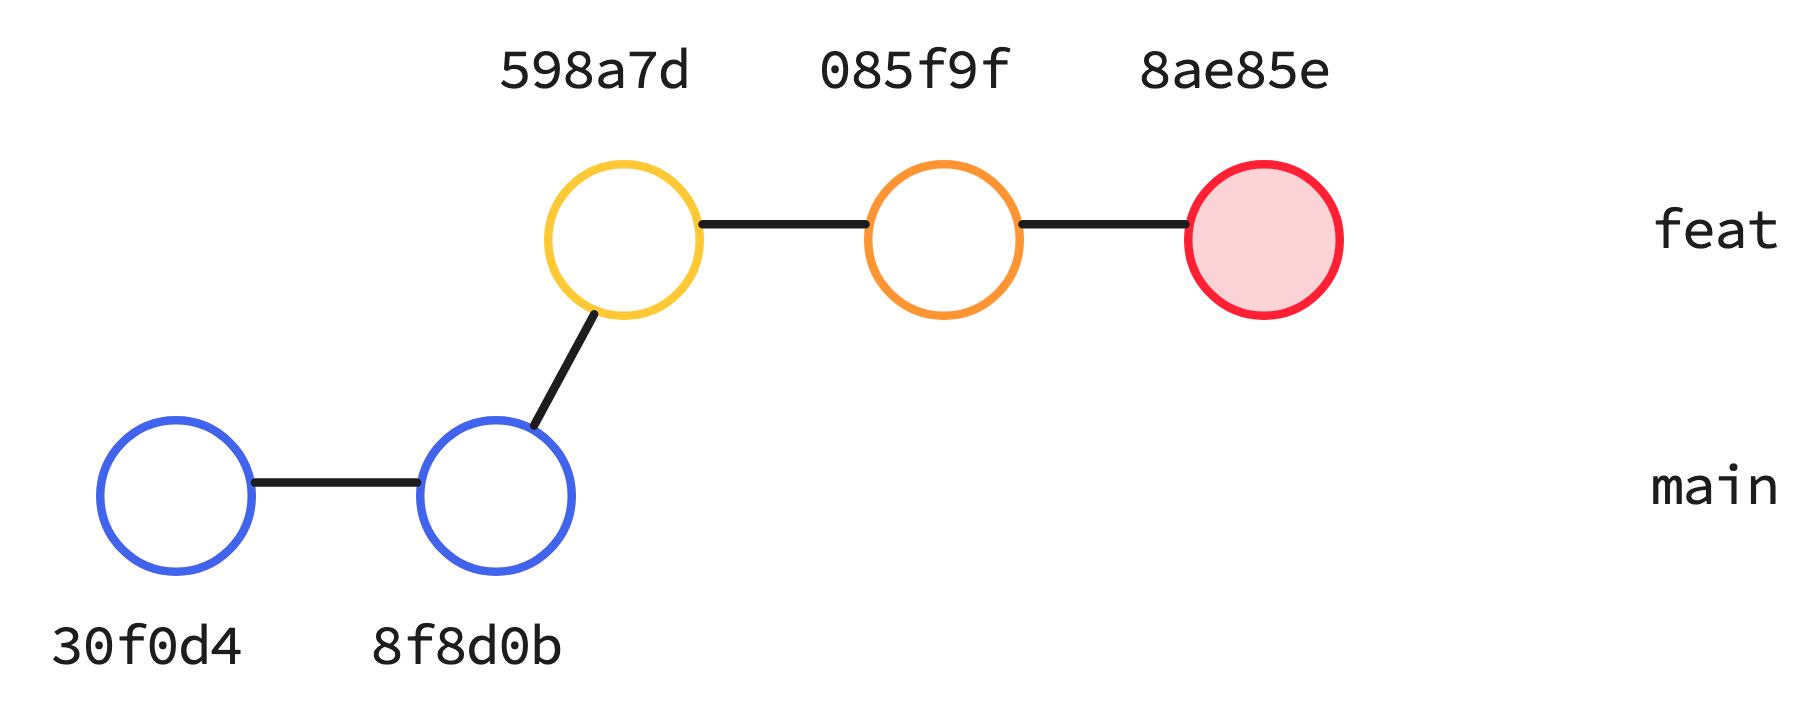
\includegraphics[width=5cm]{assets/pre-trivial.png}}
    \quad
    \subfloat{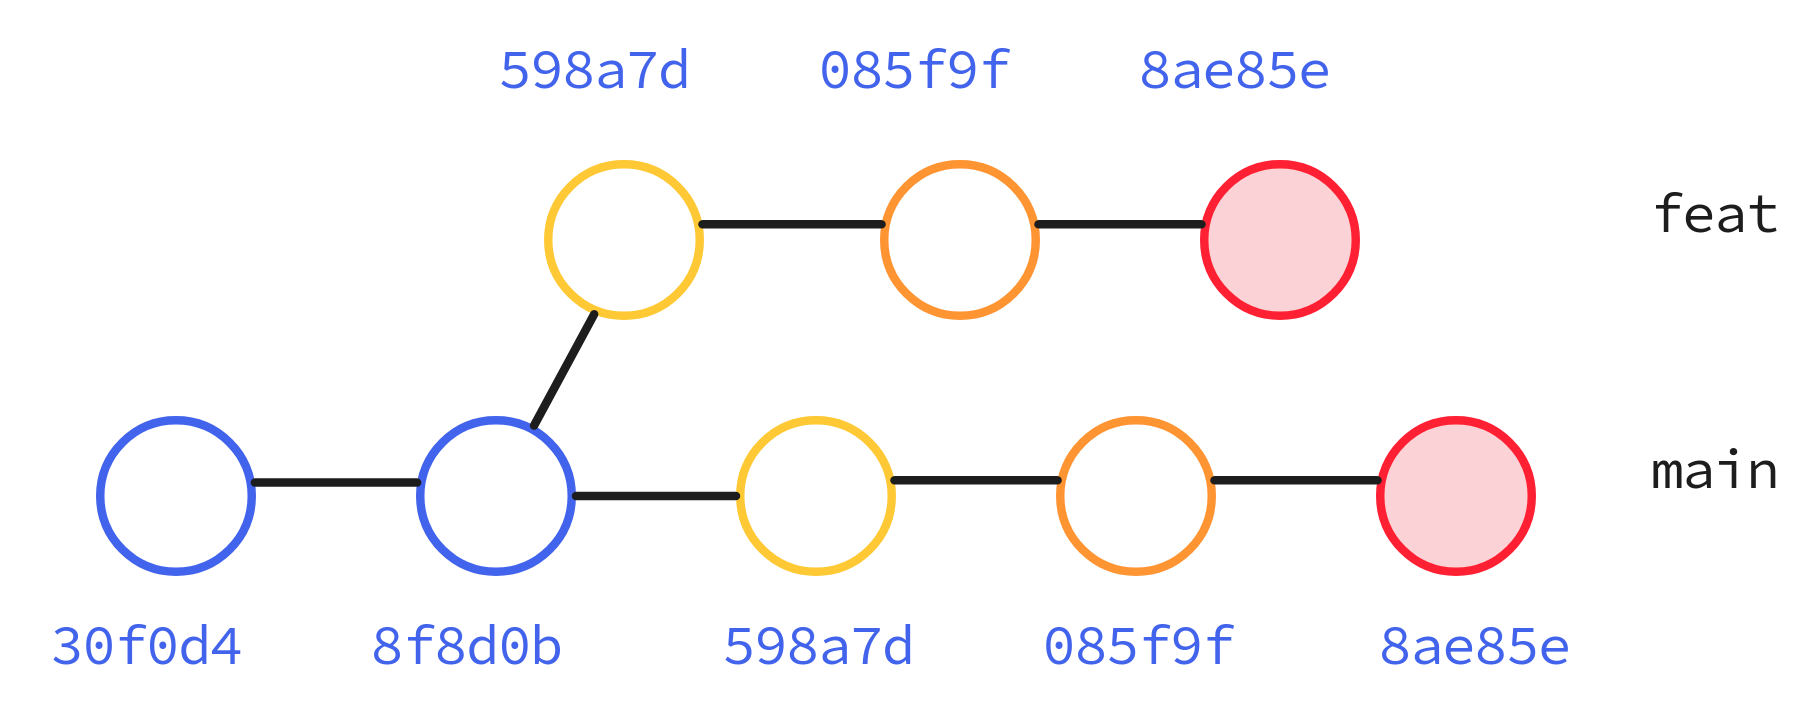
\includegraphics[width=5cm]{assets/post-trivial.png}}
    \caption{Prima e dopo un \texttt{git merge feat} o \texttt{git rebase feat}}
  \end{figure}
\end{frame}

\begin{frame}
  \label{conflict}
  \frametitle{\texttt{git merge, rebase} | Conflitti}
  Quando si vanno a unire due branch \`e possibile che si trovino conflitti tra
  i vari commit che si stanno provando ad unire. \texttt{git} si comporta in modo diverso
  in base al tipo di unione che si sta svolgendo.
  \begin{itemize}
    \item<1-> nel caso di un \texttt{merge} tutti i commit vengono applicati e 
      i file contenenti conflitti vengono segnalati all'utente. Sar\`a suo
      compito correggerli e creare il merge commit;
    \item<2-> nel caso di un \texttt{rebase} i commit vengono applicati uno ad
      uno, fermandosi quando si trovano conflitti. L'utente ha il compito di
      correggerli e far ripartire la procedura di \texttt{rebase}, iterando
      in questo modo fino al completamento.
  \end{itemize}
  In entrambi i casi il comando \texttt{git status} mostra informazioni utili
  sullo stato della procedura di unione.
\end{frame}

\begin{frame}
  \label{conflict-end}
  \frametitle{\texttt{git rebase} | Conflitti}
  Quando si incontrano conflitti durante un \texttt{rebase} si hanno in
  realt\`a tre scelte:
  \begin{itemize}
    \item<1-> correggere i conflitti e lanciare \texttt{git rebase --continue}: questo
      modificher\`a il diff del commit originale e consentir\`a di produrre un
      commit che non provoca errori con l'attuale albero di lavoro;
    \item<2-> ignorare i cambiamenti apportati da questo particolare commit (che
      sta causando i conflitti) con \texttt{git rebase --skip};
    \item<3-> annullare l'intera operazione con \texttt{git rebase --abort}
  \end{itemize}
\end{frame}

\subsection{\texttt{git stash}}
\begin{frame}
  \frametitle{\texttt{git stash [push]}}
  La famiglia di comandi \texttt{git stash} \`e usata per pulire l'albero di
  lavoro memorizzando i cambiamenti nella cosiddetta \emph{stashing area} per
  poterli riapplicare in seguito. Quest'area si comporta come una coda LIFO. \\
  Per portare i propri cambiamenti locali nell'area di \emph{stashing}:
  \begin{semiverbatim}
  \$ git stash [push]
  \end{semiverbatim}
\end{frame}

\begin{frame}
  \frametitle{\texttt{git stash pop, apply}}
  Per riportare l'ultimo set di cambiamenti nella stash nel nostro albero di
  lavoro si possono usare i comandi:
  \begin{semiverbatim}
  \$ git stash pop \text{ o } \$git stash apply
  \end{semiverbatim}
  Entrambi riportano le modifiche dell'ultimo stash sull'albero di lavoro, ma il
  \texttt{pop} rimuove anche la \emph{stash entry} dalla \emph{stashing area}.
\end{frame}

\begin{frame}
  \frametitle{\texttt{git stash} | Utilizzo}
  Un tipico utilizzo di \texttt{git stash} \`e quando si vuole effettuare un
  \texttt{pull} con risoluzione tramite \texttt{rebase}. Questo richiede che
  l'albero di lavoro sia pulito. Possiamo allora mettere da parte i cambiamenti
  locali con un \texttt{git stash}, eseguire \texttt{git pull} e riapplicare i
  nostri cambiamenti con \texttt{git stash pop}.
\end{frame}

\section{Collaborazione remota}
\begin{frame}{Perch\`e?}
  Una repository locale pu\`o essere collegata ad una \textbf{remota} per
  semplificare una serie di operazioni comuni e desiderabili:
  \begin{itemize}
    \item<1-> collaborazione tra sviluppatori, interni o esterni al proprio gruppo di lavoro;
    \item<2-> distribuzione del codice (versionamento e rilascio);
    \item<3-> backup del codice.
  \end{itemize}
\end{frame}

\subsection{\texttt{git remote}}
\begin{frame}
  \frametitle{\texttt{git remote [show]}}
  La gestione degli \emph{endpoint} remoti a cui si vuole collegare la propria
  repository avviene tramite la famiglia di comandi \texttt{git remote}.
  Per ottenere la lista dei remoti collegati ad un albero di git si pu\`o usare:
  \begin{semiverbatim}
  \$ git remote [-v]
  \end{semiverbatim}
  Applicando la flag \texttt{-v} si rende la risposta verbosa e si ottengono
  ancora pi\`u dettagli, ad esempio gli \texttt{URI} degli endpoint\footnote{
    Per ottenere ancora pi\`u informazioni si pu\`o usare il comando \texttt{git remote show <name>}
  }.
\end{frame}

\begin{frame}
  \frametitle{\texttt{git remote add, remove}}
  Per aggiungere un nuovo remoto alla repository possiamo usare il comando:
  \begin{semiverbatim}
  \$ git remote add <name> <uri>
  \end{semiverbatim}
  Il nome standard per il remoto principale \`e \emph{origin}. L'\texttt{URI}
  deve usare uno dei protoccoli accettati\footnote{Vedi:
    \href{https://stackoverflow.com/a/51112344}{\beamergotobutton{stackoverflow.com/a/51112344}}}.

    \pause
  \texttt{remove} \`e il sottocomando speculare ad \texttt{add} che consente di
  rimuovere un remoto dato il nome:
  \begin{semiverbatim}
  \$ git remote remove <name>
  \end{semiverbatim}
\end{frame}

\begin{frame}
  \frametitle{\texttt{git remote add, remove} | Nota sugli URI}
  Nella maggior parte dei servizi moderni che ospitano repository di \texttt{git}
  l'utilizzo di \texttt{HTTP(S)} come protocollo per il collegamento remoto \`e
  stato deprecato per ragioni di sicurezza. In questa guida useremo sempre
  remoti con protocollo \texttt{SSH} e voi dovreste fare altrettanto.
\end{frame}

\subsection{\texttt{git push}}
\begin{frame}
  \frametitle{\texttt{git push}}
  Una volta aggiunto un endpoint \`e possibile caricare i propri commit alla
  repository remota:
  \begin{semiverbatim}
  \$ git push [-u] [<name>]
  \end{semiverbatim} \pause
  \begin{block}{Nota}
    Dover specificare il nome del remoto ogni volta pu\`o diventare tedioso, di
    conseguenza \`e tipico identificare un remoto "di default"\footnote{Denominato \emph{upstream}}
    \emph{per ogni branch}. Questo sar\`a il remoto a cui inviare i cambiamenti
    quando \texttt{<name>} \`e omesso. La flag \texttt{-u} del comando \texttt{push}
    imposta un remoto come \texttt{upstream}.
  \end{block}
\end{frame}

\subsection{\texttt{git fetch, pull}}
\begin{frame}
  \frametitle{\texttt{git fetch}}
  Per ricevere i cambiamenti caricati ad un remoto si pu\`o usare il comando:
  \begin{semiverbatim}
  \$ git fetch [<remote>]
  \end{semiverbatim} \pause
  Quando viene omesso \texttt{<remote>} il comando scarica aggiornamenti dal
  remoto \emph{origin} o dal remoto configurato come \emph{upstream} per la
  branch attuale.
\end{frame}

\begin{frame}
  \frametitle{\texttt{git pull}}
  Quasi sempre si deisdera anche unire la branch attuale con quella remota.
  Il comando \texttt{git pull} esegue \texttt{fetch} e in seguito \texttt{merge}
  o \texttt{rebase} in base alla configurazione di \texttt{git} per riconciliare l'albero
  locale con quello remoto. \\ \pause
  \begin{itemize}
    \item nel caso non ci siano cambiamenti locali non caricati viene eseguito
      un \emph{fast-forward}\footnote{Vedi Lucido \ref{trivial}}.
    \item se ci sono cambiamenti non presenti in alcun commit che causerebbero
      conflitti il \texttt{pull} viene interrotto in attesa che essi vengano
      inseriti in un commit o rimossi.
    \item altrimenti \texttt{git} esegue \texttt{merge} o \texttt{rebase} e lascia il
      controllo all'utente in caso di conflitti come descritto nei
      Lucidi \ref{conflict}-\ref{conflict-end}.
  \end{itemize}
\end{frame}

\begin{frame}
  \frametitle{\texttt{git pull} | Nota}
  La prima volta che si esegue un pull che incontrer\`a conflitti verr\`a
  mostrato un messaggio chiedendovi di configurare il metodo di riconciliazione.
  La \emph{best practice} in questo caso \`e usare la tecnica di rebase, in
  quanto i cambiamenti in locale che hanno portato ai conflitti sono per
  definizione \emph{privati} ed \`e preferibile mantenere la storia dei commit
  lineare. Si pu\`o impostare questa opzione come default tramite:
  \begin{semiverbatim}
  \$ git config [--global] pull.rebase true
  \end{semiverbatim}
  \pause
  Se, dopo aver impostato la propria preferenza, si desidera eseguire un
  \texttt{pull} con un altro metodo di riconciliazione, si pu\`o specificare tramite:
  \begin{semiverbatim}
  \$ git pull [--rebase] [--no-rebase]
  \end{semiverbatim}
\end{frame}

\subsection{\texttt{git clone}}
\begin{frame}
  \frametitle{\texttt{git clone}}
  Per duplicare una repository remota sul proprio sistema si ha a disposizione
  il comando:
  \begin{semiverbatim}
  \$ git clone [-b <branch>] <uri>
  \end{semiverbatim}
  Dove l'\texttt{URI} \`e l'indirizzo dove \`e salvato il vostro codice.
  \pause
  \begin{block}{Consiglio}
    Per clonare una specifica branch si pu\`o usare la flag \texttt{-b}
    specificando subito dopo il nome della branch remota desiderata.
  \end{block}
\end{frame}

\begin{frame}[c]
  \centering
  It's demo time
\end{frame}

\end{document}
